\chapter{Présentation de l'entreprise}

\section{VideoStitch}
\subsection{Présentation générale}
\begin{wrapfigure}[5]{r}{7cm}
  \centering
  
\includegraphics[width=6cm]{images/videostitch.jpg}
  \caption{Logo de VideoStitch}
\end{wrapfigure}
VideoStitch est une entreprise française d'édition de logiciels, qui conçoit et 
vend des logiciels de capture, de montage, de montage, de diffusion et de lecture 
de vidéos panoramiques à 360\degree. Elle s'intéresse par extension au marché de 
la réalité virtuelle.
Son site internet est à l'adresse suivante : \url{http://www.video-stitch.com/}.\\
C'est une Société à Actions Simplifiées (SAS) basée sur Paris, qui emploie moins
d'une dizaine de personnes actuellement. La plupart ayant été embauchés il y a 
quelques mois, c'est une société en forte croissance salariale. 
Nicolas Burtey en est le président.

\subsection{Historique}
VideoStitch a été fondée par ce même Nicolas Burtey en janvier 2012.\\
Photographe diplômé de l'Ecole Lumière, s'étant fait connaître par la photo panoramique 
et la photo fish-eye, M. Burtey évolue par la suite dans le domaine de la vidéo panoramique.\\
\begin{wrapfigure}[5]{l}{6cm}
  \centering
  
\includegraphics[width=5cm]{images/loopin.png}
  \caption{Logo de Loop'In}
\end{wrapfigure}
Il crée sa société de production vidéo, Loop'In, avec laquelle il réalise une 
certain nombre de vidéos panoramiques à 360\degree pour des boites de production (publicité essentiellement). 
Des exemples de ces vidéos sont disponibles à cette adresse : \url{http://www.loop-in.com/galerie/}.
La vidéo panoramique, étant alors un procédé très jeune encore inconnu du grand public, est 
lente et difficile à réaliser: beaucoup de tâches doivent être faites de manière 
manuelle et répétitive, avec des outils inadaptés car non prévus à cette utilisation.
Si la création de photos panoramiques et à 360\degree est aisée, il manque toutefois 
un logiciel complet et mature qui permetrait l'édition et le montage de vidéos paramiques.\\
\newline
M. Burtey décide alors de créer VideoStitch pour concevoir cet outil, un logiciel 
d'édition et de montage de vidéos panoramiques : VideoStitch Studio.\\
Quand ce logiciel atteint une version stable, en 2014, VideoStitch oriente alors 
ses efforts vers un nouveau logiciel, Vahana VR, permettant cette fois-ci une réalisation 
et une diffusion en direct de vidéos panoramiques à 360\degree.\\
\newline
Le but de la société est de permettre une réalisation aisée et de qualité de vidéos 
panoramiques à 360\degree, de la capture des images à la diffusion de la vidéo finale, 
en passant par sa réalisation complète.


\section{La vidéo 360}
\subsection{Du panorama à la vidéo 360}
Une image panoramique, ou panorama, est une superposition d'images qui sont assemblées
afin de composer une vue bien plus large que ne le permet une image seule. La figure~ 
\ref{RochesterNY} présente un exemple d'assemblage d'un panorama.\\
Concrètement, avec un appareil photograhique, cela consiste à prendre plusieurs vues
successives en tournant l'appareil autour d'un axe entre deux clichés. 
Les photos obtenues forment ainsi une série d'un même sujet et doivent pouvoir chevaucher 
pour être ensuite assemblées en une image panoramique. 
Cet assemblage peut être réalisé avec directement par l'appareil, c'est le cas des 
téléphones portables, ou par un logiciel spécialisé, comme Photoshop\cite{photomerge} 
ou PTgui\cite{PTgui}.
\begin{figure}
  \centering
  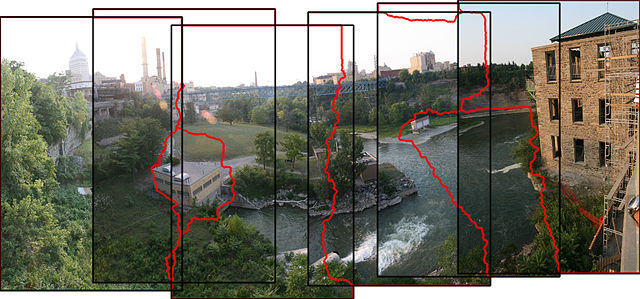
\includegraphics[width=12cm]{images/RochesterNY.jpg}
  \caption{Exemple d'assemblage de panorama avec détection des zones de chevauchement\cite{RochesterNY}}
  \label{RochesterNY}
\end{figure}
\newline
La vidéo panoramique consiste à filmer avec plusieurs caméras en même temps, chacune
capturant une partie du panorama, pour assembler les images capturées en une seule
vidéo par le même princique que la photo panoramique.\\
Avec suffisament de caméras, il est possible de couvrir un angle de prise de vue 
de 360\degree à l'horizontale et de 180\degree à la verticale. Le panorama créé
forme alors une sphère virtuelle, comme le montre la figure~\ref{rig-sphère}. 
C'est ce qu'on appelle la vidéo 360.
\begin{figure}
  \centering
  figure exemple, rig avec sphère virtuelle
\end{figure}
\newline
Cependant, comme le montre la figure~\ref{RochesterNY}, un panorama reste une image
$-$ ou une vidéo $-$, c'est-à-dire une matrice plane consistuée de pixels\footnote{Pour
 \enquote{picture element}}. Or une vidéo 360 représentant une sphère virtuelle, ou
plutôt sa surface, elle sera nécessairement une \emph{projection} de cette sphère, 
c'est-à-dire une correspondance mathématique entre cette surface en 3 dimensions 
et cette vidéo plane\cite{projection-cartographique}.\\
Dans la vidéo 360, la projection la plus utilisée est la projection équirectangulaire\cite{what-is-equirectangular}.
Un exemple en est le planisphère terrestre, où après une projection cylindrique équirectangulaire
sur la figure~\ref{projection-cylindrique} le plan est déroulé pour obtenir le 
planisphère de la figure~\ref{planisphère}.
\begin{figure}
  \centering
  \begin{minipage}{0.4\textwidth}
    \centering
    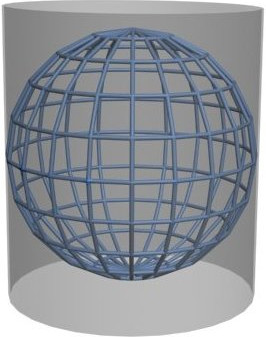
\includegraphics[width=4cm]{images/Projection-cylindrique.jpg}
    \captionof{figure}{Schéma d'une projection équirectangulaire}
    \label{projection-cylindrique}
  \end{minipage}%
  \begin{minipage}{0.6\textwidth}
    \centering
    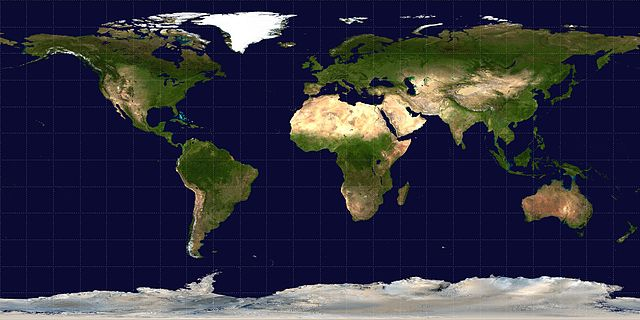
\includegraphics[width=9cm]{images/Equirectangular-projection.jpg}
    \captionof{figure}{Projection équirectangulaire de la Terre}
    \label{planisphère}
  \end{minipage}
\end{figure}
\newline
Un lecteur vidéo 360 est alors nécessaire pour lire correctement la vidéo~: 
il va reconstruire la sphère, pour y projetter le panorama et y placer le
spectateur au centre de cette sphère. Dès lors, le spectateur peut déplacer le 
regard tout autour de lui pour embrasser le panorama : on entre dans le champs de 
la réalité virtuelle\footnote{La réalité virtuelle est ici comprise dans son sens
  de \enquote{Simulation sensorielle immersive de la réalité}\cite{definition-rv}}.

\subsection{Le marché de la vidéo 360}
Si les années 2000 ont vu la démocratisation des appareils photographiques numériques,
les années 2010 voient l'émergence des caméras numériques Haute 
Définition\footnote{Définition d'image de 1920x1080 pixels} bon marché, comme les GoPro,
et des écrans 4K\footnote{Définition d'image de 4096x2160 pixels}. De plus les capacités
informatiques grand public permettent désormais de stocker et traiter plusieurs 
vidéos HD en même temps.\\
Dès lors la vidéo 360 peut se développer, son coût technique
étant accessible, et le marché, bien qu'encore restreint et méconnu du public,
est un plein développement et présente déjà de très nombreux concurrents. Jaunt,
entreprise américaine créée en mai 2013 a, par exemple, déjà levé 35 millions
de dollars de fonds d'investissement\cite{jaunt-fundings}.\\
Les grandes entreprises comme Facebook\cite{facebook-vr}, Samsung\cite{samsung-vr}, 
Microsoft\cite{microsoft-vr} ou Google\cite{google-vr} suivent de
très près ce marché, notamment pour concevoir des produits de réalité virtuelle 
ou de réalité augmentée, qui progressivement vont s'installer dans les usages
du public, tout comme l'ont fait auparavant les ordinateurs portables, les téléphones mobiles
et les tablettes numériques.\\

\section{Produits et stratégies de l'entreprise}
Par rapport à ce marché, VideoStitch se positionne aujourd'hui comme un challenger
et propose actuellement quatre produits\cite{videostitch-products}.
\subsection{VideoStitch Studio}
\label{videostitch-studio}
Logiciel de référence de Videotitch, c'est le premier logiciel stage de l'entreprise,
sortis en version stable en 2013.\\
Il permet une utilisation post-production de captures vidéos 360, c'est-à-dire 
la conception de vidéo 360. Il est intéressant de comprendre le \textit{workflow}
du logiciel : 
\subsubsection{Importation des vidéos}
Le cas le plus commun est de capturer la vidéo 360 à l'aide de 6 caméras GoPro 
installées sur une monture spécialisée comme sur la figure~\ref{rig}. 
Les caméras sont configurées pour filmer en HD, et, munies de leurs optiques 
d'origine, six sont nécessaire pour filmer toute la sphère du panorama.
\begin{figure}
  \centering
  \begin{minipage}{0.4\textwidth}
    \centering
    \caption{Une monture 360}
    \label{rig}
  \end{minipage}
  \begin{minipage}{0.6\textwidth}
    \centering
    \caption{Équirectangulaire avec angle de capture des 6 caméras} 
    \label{equirectangulaire-inputs}
  \end{minipage}
\end{figure}

\subsubsection{Synchronisation des vidéos}
Lors de la capture, les caméras sont bien souvent démarées en décalées, il s'agit
donc de resynchroniser les vidéos enregistrées.\\
Pour cela, la méthode la plus pratique est le \textit{motion},
où le logiciel analyse les mouvements de chaque vidéos, car les caméras étant fixés
sur la même monture, elles décrivent donc les même mouvement dans l'espace, mais 
en décalés sur les vidéos.

\subsubsection{Calibration}
A cette étape est reconstituée la sphère, ce qui consiste à retrouver la 
position relative de chaque caméra à la monture.\\
A un même instant des vidéos choisis par l'utilisateur, le logiciel trouve des
points de contrôle entre les images des différentes caméras, c'est-à-dire des
points identiques de la scène présent sur au moins deux images. C'est ici que les 
zones de recouvrement entre les images trouve son importance.\\
Une fois les points trouvés, les vidéos peuvent être superposées et être assemblées
\footnote{C'est ce qu'on appelle le \textit{stitch}}.
\begin{figure}
  \centering
  \label{Les 6 entrées vidéos et les points de contrôles trouvés} 
\end{figure}

\subsubsection{Correction d'exposition}
Chaque caméra ayant filmé dans une direction, elles auront chacune enregistré leur
vidéos avec différentes expositions. De même la balance des blanc peut différer
entre les vidéos. Le logiciel corrige localement ces deux paramètres pour homogéiniser
le panorama final.

\subsubsection{Stabilisation}
Le logiciel peut stabiliser le panorama, c'est-à-dire lisser les micro-mouvements 
des vidéos lors de la capture. Si la monture s'est déplacée dans l'espace lors
de l'enregistrement, cette étape est nécessaire : regarder dans un casque de réalité
virtuelle une vidéo non stabilisée est très désagréable.

\subsubsection{Exportation}
Enfin, la vidéo 360 peut être exportées, sous la forme d'un équirectangulaire, avec
possibilité d'intégrer le son d'unes des caméras.

\subsection{Vahana VR}

\subsection{VideoStitch Player}
\subsection{VideoStitch SDK}

\subsection{Stratégies}
Si VideoStitch est pendant un certain temps restée une petite start-up développant
un outil de post-production pour vidéos 360 
\footnote{VideoStitch Studio, section \ref{videostitch-studio}}, 
l'entreprise ambitionne désormais d'être le leader du marché.\\
Le marché est encore jeune, mais se décidera certainement en 2015 et s'alignera
probablement sur un leader. La technologie sera suffisament mature, et des rachats
par de grands groupe sont probable, comme cela s'est produit dans le marché de la
réalité virtuelle en 2014, avec le rachat de l'Oculus Rift par Facebook 
\cite{facebook-vr} par exemple.\\
Ce marché permettra également l'émergence de nouveaux contenus 360 pour les appareils
de réalité virtuelle, comme par exemple du cinéma ou de la télévision 360.
VideoStitch Studio et Vahana VR sont déjà des outils pertinents pour créer ces 
nouveaux types de contenus, en particulier Vahana VR pour le streaming 360 en direct.\\
\newline
Cependant d'autres pistes sont encore à développer. En effet, avec ces quatre produits
l'entreprise se destinerait actuellement à une position de service pour des entreprises de production
de vidéo 360 d'une part et à des entreprises développant des services 360 pour le
public d'une autre part. Le développement d'une solution complète incluant une 
caméra permettrait de dépasser cette position et atteindre le segment du grand public.
Cela assurerait de plus grandes rentrées d'argent et donnerait à l'entreprise des
moyens à ses ambitions.

